\documentclass[[12pt,twoside]{book}
\usepackage{_my_document_style}
\begin{document}
%
\begin{myExampleX}{Zero lift angle of a finite wing}{\ding{46}}% \ \Keyboard\ %
\label{example:Zero:Lift:Angle:Of:A:Finite:Wing}
%
\def\mySpanWingMT{26.800000}
\def\myChordRootWingMT{5.200000}
\def\myChordTipWingMT{2.340000}
\def\mySweepQuarterChordWingDEG{0.000000}
\def\mySweepQuarterChordWingRAD{0.000000}
\def\myCoeffAChordWing{-0.213433}
\def\myCoeffBChordWingMT{5.200000}
\def\myAlphaZeroLiftRootWingDEG{-3.000000}
\def\myAlphaZeroLiftTipWingDEG{-2.000000}
\def\myAlphaZeroLiftRootWingRAD{-0.052360}
\def\myAlphaZeroLiftTipWingRAD{-0.034907}
\def\myTaperRatioWing{0.450000}
\def\myTwistWingDEG{-1.500000}
\def\myTwistWingRAD{-0.026180}
\def\myTwistWingDEG{0.450000}
\def\myAreaWingMTsquared{101.036000}
\def\myCoeffAAeroTwistWingRADMT{0.001302}
\def\myCoeffATwistWingRADMT{-0.001954}
\def\myCoeffBAeroTwistWingRAD{-0.052360}
\def\myAlphaZeroLiftWingRAD{-0.033302}
\def\myAlphaZeroLiftWingDEG{-1.908046}

%
An aircraft wing has straight leading and trailing edges, wingspan $b=\SI[round-precision=1]{\mySpanWingMT}{\metre}$,
root chord $c_\mathrm{r}=\SI[round-precision=2]{\myChordRootWingMT}{\metre}$,
tip chord $c_\mathrm{t}=\SI[round-precision=2]{\myChordTipWingMT}{\metre}$
and zero sweep angle ($\Lambda_{c/4}=\SI[round-precision=0]{\mySweepQuarterChordWingDEG}{\deg}$).
Furthermore, the root profile has a zero lift angle $\alpha_{0\ell,\mathrm{r}}=\SI[round-precision=1]{\myAlphaZeroLiftRootWingDEG}{\deg}$
while the tip profile has a zero lift angle
$\alpha_{0\ell,\mathrm{t}}=\SI[round-precision=1]{\myAlphaZeroLiftTipWingDEG}{\deg}$,
with geometric twist
$\epsilon_{\mathrm{g,t}}=\SI[round-precision=1]{\myTwistWingDEG}{\deg}$. We want to calculate the zero lift angle of the wing: $\alpha_{0L}$.

\medskip
As it is known, the zero lift angle of a finite wing is the mean of the difference $\alpha_{0\ell}(Y)-\epsilon_\mathrm{g}(Y)$ (effective aerodynamic twist) weighed with the portion of the local surface $\diff{S}=c(Y)\diff{Y}$. Therefore, to calculate the integral

\[
\begin{split}
\alpha_{0L} 
  & {}= \frac{2}{S} \int_0^{b/2} 
    \Big[ 
      \alpha_{0\ell}\big(Y\big) - \epsilon_\mathrm{g}\big(Y\big) 
    \Big] \, c(Y) \diff{Y}
\end{split}
\]
the laws of variation along the wingspan have to be reconstructed:%
\begin{inparaenum}[(\itshape i\normalfont)]
\item
of the chord,
\item
of section zero lift angle, 
\item
of the geometric section keying.
\end{inparaenum}
In absence of specific indications, it can be assumed that the last two laws are linear. The linear law applies to section chords
$c \big( Y \big) = A_c \, Y + B_c$ 
with
\[
A_c
  = \frac{c_\mathrm{t} - c_\mathrm{r}}{b/2}
  = 
    2 \frac{
      \SI[round-precision=2]{\myChordTipWingMT}{\metre} - \SI[round-precision=2]{\myChordRootWingMT}{\metre}
    }{
      \SI[round-precision=2]{\mySpanWingMT}{\metre}
    }
  = \mathunderline{mydarkblue}{ \SI[round-precision=3]{\myCoeffAChordWing}{} }
\]
\[
B_c
  = c_\mathrm{r}
  = \mathunderline{mydarkblue}{ \SI[round-precision=2]{\myCoeffBChordWingMT}{\metre} }
\]
So
\[
c \big( Y \big) = A_c \, Y + B_c
  = \SI[round-precision=3]{\myCoeffAChordWing}{} \, Y
    + \SI[round-precision=2]{\myCoeffBChordWingMT}{\metre}
\]
The linear law holds for the angles of zero lift section $\alpha_{0\ell} \big( Y \big) = A_{\alpha} \, Y + B_{\alpha}$ 
with
\[
A_{\alpha}
  = \frac{\alpha_{0\ell,\mathrm{t}} - \alpha_{0\ell\mathrm{r}}}{b/2}
  = 
    2 \frac{
      \SI[round-precision=4]{\myAlphaZeroLiftTipWingRAD}{\radian} 
        - ( \SI[round-precision=4]{\myAlphaZeroLiftRootWingRAD}{\radian} )
    }{
      \SI[round-precision=2]{\mySpanWingMT}{\metre}
    }
  = \mathunderline{mydarkblue}{ \SI[round-precision=5]{\myCoeffAAeroTwistWingRADMT}{\radian/\metre} }
\]
\[
B_{\alpha}
  = \alpha_{0\ell,\mathrm{r}}
  = \mathunderline{mydarkblue}{ \SI[round-precision=4]{\myAlphaZeroLiftRootWingRAD}{\radian} }
\]
therefore
\[
\alpha_{0\ell} \big( Y \big) = A_{\alpha} \, Y + B_{\alpha}
  = (\SI[round-precision=5]{\myCoeffAAeroTwistWingRADMT}{\radian/\metre}) \, Y
    \SI[round-precision=4]{\myAlphaZeroLiftRootWingRAD}{\radian}
\]
The linear law applies to the geometric twist angles of section
$\epsilon_\mathrm{g} \big( Y \big) = A_{\epsilon} \, Y + B_{\epsilon}$ 
with
\[
A_{\epsilon}
  = \frac{\epsilon_{\mathrm{g,t}} - \epsilon_{\mathrm{g,r}}}{b/2}
  = 
    2 \frac{
      \SI[round-precision=4]{\myTwistWingRAD}{\radian} 
    }{
      \SI[round-precision=2]{\mySpanWingMT}{\metre}
    }
  = \mathunderline{mydarkblue}{ \SI[round-precision=5]{\myCoeffATwistWingRADMT}{\radian/\metre} }
\]
\[
B_{\epsilon}
  = \mathunderline{mydarkblue}{ \SI[round-precision=0]{0}{\radian} }
\]
therefore
\[
\epsilon_\mathrm{g} \big( Y \big) = A_{\epsilon} \, Y + B_{\epsilon}
  = (\SI[round-precision=5]{\myCoeffATwistWingRADMT}{\radian/\metre}) \, Y
\]
The assigned wing has a taper ratio
\[
\lambda
  =\frac{c_\mathrm{t}}{c_\mathrm{r}}
  =\frac{\SI[round-precision=2]{\myChordTipWingMT}{\metre}}{\SI[round-precision=2]{\myChordRootWingMT}{\metre}}
  =\mathunderline{mydarkblue}{ \SI[round-precision=2]{\myTaperRatioWing}{} }
\]
and a wing surface
\[
\begin{split}
S & {}= \frac{b}{2} \, c_\mathrm{r} \, \big( 1 + \lambda \big) \\
  & {}=
    \num{0.5} \cdot \SI[round-precision=1]{\mySpanWingMT}{\metre}
      \cdot \SI[round-precision=2]{\myChordRootWingMT}{\metre}
      \cdot \big( 1 + \SI[round-precision=2]{\myTaperRatioWing}{} \big) 
    = \mathunderline{mydarkblue}{ \SI[round-precision=1]{\myAreaWingMTsquared}{\metre^2} }
\end{split}
\]
At this point it is possible to calculate the angle of zero lift
\[
\begin{split}
\alpha_{0L} 
  & {}= \frac{2}{S} \int_0^{b/2} 
    \Big[ 
      \alpha_{0\ell}\big(Y\big) - \epsilon_\mathrm{g}\big(Y\big) 
    \Big] \, c(Y) \diff{Y}
\\[3pt]
  & {}= \frac{2}{S} \int_0^{b/2} 
    \bigg[ \Big( A_{\alpha} \, Y + B_{\alpha} \Big) - A_{\epsilon} \, Y \bigg] \Big( A_c Y + B_c \Big)
      \diff{Y}
\end{split}
\]
The value of the definite integral is easily obtained by substituting the values in the integrating function of the previously calculated coefficients. We have
\[
\begin{split}
\alpha_{0L} 
%
   & ={}
     \frac{2}{ \SI[round-precision=1]{\myAreaWingMTsquared}{\metre^2} }
     \int_{\SI{0}{m}}^{
       \calcSI[round-precision=1,fixed-exponent=0,scientific-notation=fixed]{0.5*\mySpanWingMT}{\metre}
     }
     \Big[ 
       %\Big( 
         % A_{\alpha} \, Y + B_{\alpha} 
         \SI[round-precision=5]{\myCoeffAAeroTwistWingRADMT}{\radian/\metre} \; Y
           \SI[round-precision=4]{\myAlphaZeroLiftRootWingRAD}{\radian}
       %\Big) 
\\
  & \rule{0.3\linewidth}{0pt}% --> SPACER
       % - A_{\epsilon} \, Y 
       - ( \SI[round-precision=5]{\myCoeffATwistWingRADMT}{\radian/\metre} ) \; Y
     \Big] 
     \Big( 
       \SI[round-precision=3]{\myCoeffAChordWing}{} \; Y
         + \SI[round-precision=2]{\myCoeffBChordWingMT}{\metre}
       \Big) \diff{Y}
%
\\
  & {}= 
     \frac{2}{ \SI[round-precision=1]{\myAreaWingMTsquared}{\metre^2} }
     \int_{\SI{0}{m}}^{
       \calcSI[round-precision=1,fixed-exponent=0,scientific-notation=fixed]{0.5*\mySpanWingMT}{\metre}
     }
     \Big( 
%
    \calcSI[round-precision=6,fixed-exponent=0,scientific-notation=fixed]{
      (\myCoeffAAeroTwistWingRADMT)*(\myCoeffAChordWing)
    }{\radian/\metre}
    \; Y^2
    +
    \calcSI[round-precision=4,fixed-exponent=0,scientific-notation=fixed]{
      (\myCoeffBAeroTwistWingRAD)*(\myCoeffAChordWing)
    }{\radian}
    \; Y
    -
    \calcSI[round-precision=6,fixed-exponent=0,scientific-notation=fixed]{
      (\myCoeffATwistWingRADMT)*(\myCoeffAChordWing)
    }{\radian/\metre}
    \; Y^2
%
\\
  & 
    \rule{0.25\linewidth}{0pt}% --> SPACER
%
    +
    \calcSI[round-precision=5,fixed-exponent=0,scientific-notation=fixed]{
      (\myCoeffAAeroTwistWingRADMT)*(\myCoeffBChordWingMT)
    }{\radian}
    \; Y
%
    + (
    \calcSI[round-precision=3,fixed-exponent=0,scientific-notation=fixed]{
      (\myCoeffBAeroTwistWingRAD)*(\myCoeffBChordWingMT)
    }{\radian\,\metre}
    )
%
    - (
    \calcSI[round-precision=4,fixed-exponent=0,scientific-notation=fixed]{
      (\myCoeffATwistWingRADMT)*(\myCoeffBChordWingMT)
    }{\radian}
    )
    \; Y
%
    \Big) \diff{Y}
\end{split}
\]
Solving the definite integral we obtain
\[
\begin{split}
\alpha_{0L} 
%
  & {}= 
%
    \frac{2}{ \SI[round-precision=1]{\myAreaWingMTsquared}{\metre^2} }
%
    \bigg[
    \calcSI[round-precision=6,fixed-exponent=0,scientific-notation=fixed]{
      (\myCoeffAAeroTwistWingRADMT)*(\myCoeffAChordWing)
    }{\radian/\metre}
    \; \frac{Y^3}{3}
    +
    \calcSI[round-precision=4,fixed-exponent=0,scientific-notation=fixed]{
      (\myCoeffBAeroTwistWingRAD)*(\myCoeffAChordWing)
    }{\radian}
    \; \frac{Y^2}{2}
    -
    \calcSI[round-precision=6,fixed-exponent=0,scientific-notation=fixed]{
      (\myCoeffATwistWingRADMT)*(\myCoeffAChordWing)
    }{\radian/\metre}
    \; \frac{Y^3}{3}
\\[2pt]
  & 
    \rule{0.20\linewidth}{0pt}% --> SPACER
%
    +
    \calcSI[round-precision=5,fixed-exponent=0,scientific-notation=fixed]{
      (\myCoeffAAeroTwistWingRADMT)*(\myCoeffBChordWingMT)
    }{\radian}
    \; \frac{Y^2}{2}
%
    + (
    \calcSI[round-precision=3,fixed-exponent=0,scientific-notation=fixed]{
      (\myCoeffBAeroTwistWingRAD)*(\myCoeffBChordWingMT)
    }{\radian\,\metre}
    )
    \; Y
%
    - (
    \calcSI[round-precision=4,fixed-exponent=0,scientific-notation=fixed]{
      (\myCoeffATwistWingRADMT)*(\myCoeffBChordWingMT)
    }{\radian}
    )
    \; \frac{Y^2}{2}
%
    \bigg]_{\SI{0}{m}}^{
      \calcSI[round-precision=1,fixed-exponent=0,scientific-notation=fixed]{0.5*\mySpanWingMT}{\metre}
    }
%
\\[2pt]
  & {}= \mathunderline{mydarkblue}{ \SI[round-precision=4]{\myAlphaZeroLiftWingRAD}{\radian} }
  = \mathunderline{mydarkblue}{ \SI[round-precision=2]{\myAlphaZeroLiftWingDEG}{\deg} }
\end{split}
\]
It is observed that the result obtained corresponds to an intermediate value between the angle $\alpha_{0\ell,\mathrm{r}}$
of zero lift of the root ($\SI[round-precision=1]{\myAlphaZeroLiftRootWingDEG}{\deg}$)
and the difference
\[
\alpha_{0\ell,\mathrm{t}}-\epsilon_\mathrm{t}
  = \SI[round-precision=1]{\myAlphaZeroLiftTipWingDEG}{\deg}
    -( \SI[round-precision=1]{\myTwistWingDEG}{\deg} ) 
  = \calcSI[round-precision=1,fixed-exponent=0,scientific-notation=fixed]{
    \myAlphaZeroLiftTipWingDEG - (\myTwistWingDEG)
  }{deg}
\]
between the angle of zero lift of the tip and the geometric twist angle of the tip. The value of $\alpha_{0L}$ is closer to that of
$\alpha_{0\ell,\mathrm{r}}$ due to the tapering.
%
\begin{figure}[t]%[H]%[!htbp]
  \centering
  %\checkoddpage
  %\centering
    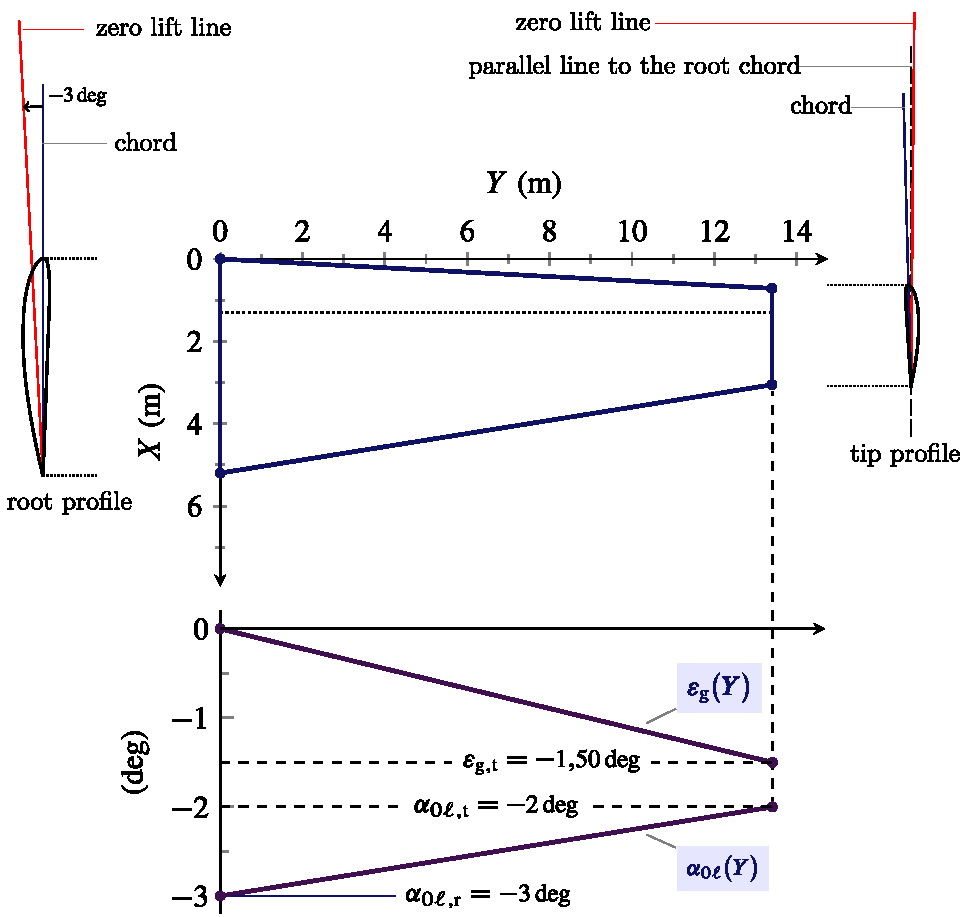
\includegraphics[width=0.78\textwidth]{Chapter_2/zero_lift_angle_of_a_finished_wing/wing_alpha_zero_lift_basic_1_drawing.pdf}
  \caption{\finalhyphendemerits=1000
    Planform of the cranked wing
 assigned in the example~\ref{example:Zero:Lift:Angle:Of:A:Finite:Wing}.
    The linear laws of geometric twist angle $\epsilon_\mathrm{g}$, and zero lift angle of section $\alpha_{0\ell}$ are represented.
   On the left there is the diagram of the root profile with its zero lift line and its chord. This is the reference line for the angles $\epsilon_\mathrm{g}(Y)$. 
    The tip profile is drawn on the right, splined by an angle
    $\epsilon_{\mathrm{g,t}}=\epsilon_\mathrm{g}(\frac{1}{2}b)$.%  
    }
  \label{fig:Zero:Lift:Basic:1}%
\end{figure}
%
\end{myExampleX}
\end{document}